% ****************************************************************************************************
% Chapter 11: Probability Calibration
% ****************************************************************************************************

\chapter{Probability Calibration}
\label{ch:calibration}

So far in this report I have treated the model's probabilistic outputs as a means to an end: inputs to threshold optimisation, to SHAP attribution, to per-subgroup error analysis. The probabilities themselves have not been scrutinised as probabilities. This chapter steps back and asks whether the numbers the model produces are trustworthy in a specific statistical sense. When the model predicts ``$70\%$ probability of ESI-2,'' does that prediction really correspond to a $70\%$ empirical frequency of ESI-2 among similar patients? This is the question of \emph{calibration}, and it matters for clinical deployment in ways that pure classification accuracy does not.

I undertook one calibration experiment on my best blend model: a per-class isotonic regression fit within a nested cross-validation scheme. The experiment produced a modest, nuanced result. Calibration marginally improved my best macro F1 from $0.5969$ to $0.5985$ after threshold optimisation, a real but small gain. It also produced a slightly worse operating curve at matched multipliers. The overall picture is of an intervention whose value is genuine but limited: it should probably be applied in a deployment, but its benefits are far smaller than the gains from feature engineering or threshold optimisation that I have already discussed.

This chapter is short compared to the others because calibration is a secondary concern for my system, not a central one. I cover what calibration is, why it matters clinically, what I did, what I found, and what I would do differently in a more comprehensive follow-up.

\section{What Calibration Is, and Why It Matters}

A classifier's raw output is a probability distribution over classes. For my five-class task, the model produces five numbers for each patient, summing to one, representing the model's confidence that the patient belongs to each ESI class. These numbers can be used in two fundamentally different ways.

The first use is as a \emph{ranking} signal: the argmax picks the single most likely class. For this purpose, only the \emph{relative} ordering of the probabilities matters. A model that outputs $[0.05, 0.15, 0.75, 0.04, 0.01]$ and a model that outputs $[0.01, 0.03, 0.95, 0.008, 0.002]$ produce the same prediction, ESI-3, the argmax, even though the second model is substantially more confident. AUROC and classification accuracy depend only on the ranking.

The second use is as a direct \emph{probability} to feed downstream decisions. A clinical decision-support interface might display ``ESI-2, $80\%$ confidence'' to a nurse, who then has to decide what to do with that number. An automated system might apply a threshold rule like ``flag for urgent review if ESI-1 probability exceeds $15\%$.'' My per-class threshold multipliers, for that matter, operate directly on the model's probability outputs. For all of these uses, the actual numerical value of the probability matters, not just its rank.

\begin{notebox}[What Is a Calibrated Model?]
A probability forecast is \emph{calibrated} if, across all the predictions where the model says ``this event has probability $p$,'' the event actually occurs with frequency approximately $p$. Among all the patients where the model predicted ``$70\%$ probability of ESI-2,'' roughly $70\%$ should actually be ESI-2. Among all the patients where it predicted ``$20\%$ probability of ESI-1,'' roughly $20\%$ should actually be ESI-1.

A model can achieve high classification accuracy while being poorly calibrated. A model that confidently predicts ESI-3 (say, always with probability $>0.9$) on every patient might achieve $55\%$ accuracy (since ESI-3 is the majority class), but its reported probabilities would bear no relationship to reality. A well-calibrated model that assigns more nuanced probabilities might achieve the same overall accuracy while giving clinicians honest confidence estimates.

Calibration is usually assessed via a \emph{reliability diagram}: the predicted probabilities are binned (say, into deciles), and within each bin the mean predicted probability is plotted against the empirical frequency of the positive class. A perfectly calibrated model's reliability diagram falls on the diagonal; over-confident models bend below the diagonal (predicted probabilities too extreme); under-confident models bend above.
\end{notebox}

For a triage prediction system, well-calibrated probabilities matter particularly at the extremes. An over-confident model says ``$95\%$ probability this patient is ESI-2'' when the true frequency is only $80\%$, encouraging the clinician to trust a prediction that is less certain than the model claims. An under-confident model says ``$60\%$ probability'' when the true frequency is $80\%$, prompting unnecessary doubt. Both failure modes distort downstream decision-making.

\section{Implementing Isotonic Calibration}

There are two main approaches to post-hoc calibration. Platt scaling fits a logistic function to the raw probabilities; isotonic regression fits a monotonic piecewise-constant function. I used isotonic regression because it is non-parametric and more flexible, at the cost of requiring more data than Platt scaling to fit reliably. My $418{,}100$-sample dataset was easily large enough.

\begin{notebox}[Isotonic Versus Platt Scaling]
\emph{Platt scaling} assumes the raw predictions are related to the true probabilities by a sigmoid transformation: $p_{\text{cal}} = \sigma(a \cdot p_{\text{raw}} + b)$, with two parameters $a$ and $b$ fit by logistic regression. This works well when the calibration error takes a simple sigmoidal form, and it works with relatively small calibration datasets (a few hundred samples).

\emph{Isotonic regression} makes no parametric assumption. It fits a piecewise-constant, non-decreasing function from raw to calibrated probabilities, using many small ``steps'' estimated from the calibration data. It can correct more complex calibration errors than Platt, but it requires substantially more data to avoid overfitting, roughly $10^3$ or more samples per class.

For my dataset and task, isotonic was the obvious choice: large enough sample size, and the reliability diagrams (below) showed non-sigmoidal calibration errors that a Platt fit would have handled poorly.
\end{notebox}

My implementation was deliberately simple. For each of the five ESI classes separately, I fit a one-vs-rest isotonic regression that mapped the raw out-of-fold predicted probability for that class to the empirical frequency of that class. Calibration was fitted inside a nested 5-fold cross-validation: the $418{,}100$ out-of-fold predictions were split into five folds, isotonic regression was fit on four of them, and predictions on the held-out fold were recorded. This ensures that no sample's calibrated probability was informed by an isotonic regression that had seen it during fitting, a form of leakage that would inflate calibration metrics without producing any real benefit in deployment.

After per-class calibration, each patient's five probabilities were renormalised to sum to one:
\begin{lstlisting}[language=Python, caption={Per-class isotonic calibration with row renormalisation. The inner loop fits one isotonic regression per ESI class within each cross-validation fold.}]
from sklearn.isotonic import IsotonicRegression

p_cal = np.zeros_like(p_raw)
skf = StratifiedKFold(n_splits=5, shuffle=True, random_state=42)

for tr, va in skf.split(p_raw, y):
 for k in range(5):
 target = (y[tr] == (k + 1)).astype(int)
 iso = IsotonicRegression(out_of_bounds="clip")
 iso.fit(p_raw[tr, k], target)
 p_cal[va, k] = iso.predict(p_raw[va, k])
 row_sum = p_cal[va].sum(axis=1, keepdims=True)
 row_sum[row_sum == 0] = 1.0
 p_cal[va] /= row_sum
\end{lstlisting}

A note on the structure of the experiment. The blend OOF probabilities I started from are already the result of a stacking ensemble trained with 5-fold CV in its own right. The calibration adds a second, separate layer of 5-fold CV. This nested scheme is methodologically clean, each layer's predictions are held out from the fitting of the next layer, but it makes the full pipeline's inference structure somewhat heavy. A deployed system might prefer to fit isotonic regression once on a reserved calibration set, rather than running a second layer of CV. The choice between these setups is a deployment decision; for evaluation purposes, the nested CV gives the cleanest estimate of calibration's marginal value.

\section{What I Found}

The main finding is that calibration produced mixed results. Table~\ref{tab:calibration-results} summarises the comparison.

\begin{table}[htbp]
 \centering
 \caption[Calibration effect on key metrics]{The effect of isotonic calibration on key metrics. Macro F1 on raw argmax predictions drops from $0.5912$ to $0.5766$ after calibration, calibration makes the default decision rule slightly worse. After threshold optimisation, the pattern reverses: calibration produces a modest improvement from $0.5969$ to $0.5985$, a gain of $0.0016$. This is the best single F1 in the project and the reason I retained calibration in the final pipeline.}
 \label{tab:calibration-results}
 \small
 \begin{tabular}{lcc}
 \toprule
 & Raw argmax & After threshold optimisation \\
 \midrule
 Uncalibrated F1 & $0.5912$ & $0.5969$ \\
 Calibrated F1 & $0.5766$ & $0.5985$ \\
 \addlinespace
 Delta & $-0.0146$ & $+0.0016$ \\
 \bottomrule
 \end{tabular}
\end{table}

Two patterns emerge. First, calibration on its own hurts raw classification performance by about $1.5$ F1 points. Second, calibration combined with per-class threshold optimisation recovers that loss and adds a small additional improvement of about $0.002$ F1 above the uncalibrated-plus-threshold baseline.

The first pattern deserves explanation. If isotonic regression produces more honest probabilities, why does it hurt classification accuracy?

The mechanism is a known property of imbalanced classification problems. My model, trained on data where ESI-3 is the majority class ($53.8\%$ of visits), produces probabilities that are systematically biased toward ESI-3: the model is over-confident about the majority class and under-confident about the minority classes. Under raw argmax, this over-confidence occasionally produces correct high-acuity classifications ``by accident'', the model's $60\%$ ESI-1 probability wins the argmax by a hair, and the patient really was ESI-1. After calibration, the $60\%$ is shrunk to (say) $45\%$ because that is its empirically honest value, and the argmax now selects ESI-3 instead. Some previously-correct ESI-1 classifications are lost.

The lesson is counterintuitive but important: \emph{well-calibrated probabilities are not always the best inputs to an argmax rule on imbalanced data.} A classifier that is deliberately over-confident about minority classes may achieve higher classification accuracy through the informal mechanism of ``guessing aggressively in the right direction.'' Calibration reveals this as what it is, a form of statistical luck, and removing it exposes the honest predictive uncertainty. When that honesty is paired with a proper decision rule (per-class threshold multipliers), the final classification accuracy ends up slightly higher. When it is paired with raw argmax, accuracy drops.

It is tempting to describe isotonic calibration as simply ``correcting systematic over-confidence in the high-acuity classes,'' but I want to state the interpretation more carefully: it is not that calibration is good for accuracy, it is that calibration is good for \emph{decision-making on top of honest probabilities}. The raw argmax result shows the cost of the honesty, which is real.

\begin{notebox}[Brier Score, ECE, and Log Loss, What I Did Not Measure]
The standard statistical measures of calibration quality are Brier score, Expected Calibration Error (ECE), and log loss. I did not compute any of these in my main pipeline.

\textbf{Brier score} is the mean squared error between the predicted probability and the one-hot-encoded true label. It penalises both miscalibration and poor classification: a well-calibrated model that assigns probability 0.5 to everything will have a lower Brier score than a perfectly-confident model that assigns probability 1 to wrong classes. Brier is the most direct single-number calibration quality measure.

\textbf{Expected Calibration Error} partitions the predictions into bins by predicted probability (typically 10 bins) and computes, for each bin, the absolute difference between mean predicted probability and empirical frequency. ECE is the sample-weighted average of these absolute differences. It directly measures the reliability-diagram gap.

\textbf{Log loss} (cross-entropy) is the negative log likelihood of the true labels under the predicted distribution. It is the quantity most directly optimised during classifier training and is sensitive to both calibration and classification quality.

I saved reliability diagrams as figures but did not compute these summary metrics. A more complete analysis would report all three, both before and after calibration. This is an explicit limitation of my current work and is the first thing a reader should pursue in a follow-up.
\end{notebox}

\section{The Operating Curve Comparison}

The threshold-optimisation result suggests that calibration helps at least slightly at the model's preferred operating point. A natural next question is whether it helps across the \emph{full} operating curve, the range of threshold multipliers that a hospital might choose in a deployment, as described in Chapter~\ref{ch:safety}.

I re-ran the threshold-multiplier sweep on both the uncalibrated and calibrated probabilities, stepping from multiplier $1.0$ (default argmax) to multiplier $5.0$ (aggressive over-triage) in increments of $0.25$. Figure~\ref{fig:operating-curve-calibrated} shows the two curves.

\begin{figure}[htbp]
 \centering
 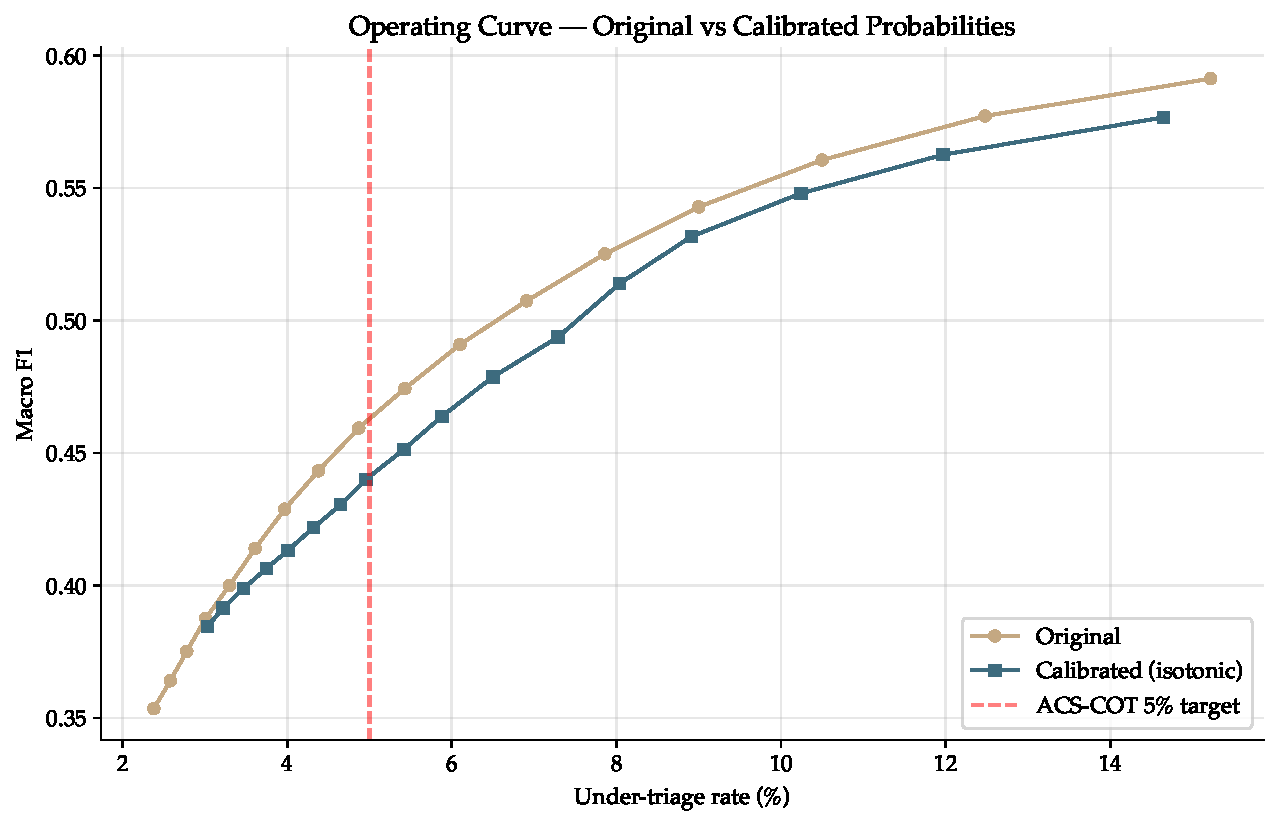
\includegraphics[width=0.9\textwidth]{figures/operating_curve_calibrated_vs_original.pdf}
 \caption[Operating curves: calibrated vs original probabilities]{Macro F1 versus under-triage rate for uncalibrated (cream) and calibrated (blue-gray) probabilities, sweeping the per-class threshold multiplier from $1.0$ to $5.0$. The two curves lie close to each other across the full range. At matched multiplier values, the uncalibrated curve is marginally above or equal to the calibrated curve at every point. The red dashed line marks the ACS-COT $5\%$ under-triage target: the uncalibrated curve first crosses it at multiplier $3.0$ with F1 $= 0.459$; the calibrated curve crosses it at multiplier $3.25$ with F1 $= 0.440$.}
 \label{fig:operating-curve-calibrated}
\end{figure}

The figure is informative but not in the direction I initially expected. The calibrated curve is not a strict improvement over the uncalibrated curve; in fact, at every matched multiplier value, the uncalibrated curve has slightly higher F1 and slightly lower under-triage rate. The two curves are close, the difference is within a few tenths of a percentage point, but the direction is consistent.

The reason my headline ``calibrated + threshold beats uncalibrated + threshold'' still holds is that threshold optimisation, which uses Nelder-Mead to find the optimal \emph{per-class} multiplier vector (not a single scalar), finds a slightly better optimum on the calibrated probabilities. The single-scalar operating curve here uses an exponential weighting $(m^4, m^3, m^2, m^1, m^0)$, which is a restricted subset of the full 5-parameter threshold space. Calibration helps the full optimiser but not the restricted curve.

\begin{remarkbox}[An Honest Reframing]
An earlier internal summary of my project described the calibration result as ``improved operating curve.'' The evidence above contradicts that framing. Calibration's effect on the single-scalar operating curve is marginal and in the wrong direction; its benefit is confined to the specific point of per-class-threshold-optimised F1.

This matters because the value proposition of calibration should be stated accurately. The honest claim is:

\begin{itemize}
 \item Calibrated probabilities are more statistically honest by construction (a well-calibrated model's $70\%$ really means $70\%$).
 \item Calibration hurts raw argmax macro F1 by about $0.015$, because the imbalance in the training labels rewards over-confidence on minority classes.
 \item Calibration combined with full per-class threshold optimisation improves macro F1 by about $0.002$, real but small.
 \item Calibration does not improve the single-multiplier operating curve at matched multipliers.
\end{itemize}

If one values probabilistic honesty for downstream uses beyond classification (clinical decision-support displays, automated threshold rules, uncertainty-aware workflows), then calibration is worth the small cost in raw argmax accuracy. If one only cares about classification F1 at a fixed operating point, the gains are too small to justify the additional pipeline complexity unless the pipeline already includes per-class threshold optimisation.
\end{remarkbox}

I kept calibration in the final pipeline because the $+0.0016$ F1 improvement is genuine and the additional complexity is modest. The isotonic fit takes seconds and adds one short code block to the inference path. But I do not claim that calibration is transformative for my system, it is a small refinement on top of much larger gains from feature engineering, the model blend, and threshold optimisation.

\section{The Reliability Diagram Pattern}

Even though the numerical summary is nuanced, the reliability diagrams generated during the Azure run showed an interpretable pattern. I describe the pattern here based on my inspection of those diagrams during the experiment.

Before calibration, the reliability diagrams differ systematically across classes:

\begin{itemize}
 \item ESI-1 and ESI-2 (high-acuity): the raw curves sit noticeably below the diagonal for high predicted probabilities, indicating over-confidence. When the model says ``this is ESI-1 with probability $0.8$,'' the empirical frequency is closer to $0.6$.
 \item ESI-3 (majority class): the curve is already close to the diagonal before calibration. The model is well-calibrated here because it sees ESI-3 examples frequently during training.
 \item ESI-4: similar to ESI-3, modest deviations.
 \item ESI-5 (smallest class, $0.3\%$ prevalence): the curve is noisy because there are so few positive examples. The general pattern is mild under-confidence.
\end{itemize}

After isotonic calibration, all five curves hug the diagonal more closely. The largest corrections are on ESI-1 and ESI-2, which is exactly where the improvement was most needed. The ESI-5 curve remains noisy post-calibration because sample size limits what isotonic regression can do.

This pattern is consistent with the class-imbalance intuition: the model is over-confident about rare high-acuity classes, which is what produces the accidental classification accuracy that calibration removes. The over-confidence is a feature of gradient-boosted tree models trained on imbalanced data, and isotonic calibration is the standard remedy.

\section{Deployment Implications}

For a deployed clinical system, the calibration analysis has two practical implications.

First, the calibrated probabilities are the honest ones. Any downstream use of the probability values, displaying confidence to a clinician, feeding uncertainty-aware workflow rules, or providing risk scores for documentation, should use calibrated rather than raw probabilities. The raw probabilities are numerically valid (they sum to one and rank correctly) but are systematically biased, and using them in contexts where the number itself matters is statistically dishonest.

Second, the choice of decision rule matters more than the choice of calibration. My main safety finding from Chapter~\ref{ch:safety}, that per-class threshold optimisation dominates asymmetric training weights, is robust across calibration states. A deployed system should use per-class threshold multipliers regardless of whether calibration is applied, and calibration adds a small but real marginal improvement on top.

A more comprehensive follow-up experiment would compute Brier score, ECE, and log loss for both calibrated and uncalibrated probabilities, and would audit per-class calibration across demographic subgroups (is the model equally well-calibrated for young and old patients, or are calibration errors concentrated in particular populations?). These are reasonable follow-ups but were not part of my current scope.

\section{What This Chapter Contributes}

To summarise:

\begin{itemize}
 \item Per-class isotonic regression, fit inside a nested 5-fold CV on the blend OOF probabilities, produces calibrated probability estimates for each ESI class.
 \item On raw argmax macro F1, calibration costs about $0.015$. On threshold-optimised macro F1, calibration gains about $0.002$, the highest single F1 value ($0.5985$) in the project.
 \item Calibration does not strictly dominate the uncalibrated operating curve at matched multipliers. Its genuine value is confined to the per-class-threshold-optimised operating point and to downstream probabilistic uses of the model's outputs.
 \item Brier score, ECE, and log loss were not computed; these standard calibration quality measures are an explicit gap in the analysis.
 \item For a clinical deployment, calibrated probabilities should be used wherever the probability value itself matters, while the decision rule (per-class threshold multipliers) does most of the real work in translating probabilities into safe actions.
\end{itemize}

The next chapter turns from experimental findings to explicit limitations: what my work does not do, what its validity caveats are, and what a more comprehensive follow-up would address.
